\section{CHAPTER 9: FLOW METERS}

\subsection{Overview:}

A flow meter in a steam system is a device operated to assess the rate
of steam flow through pipelines or channels. It provides essential data
for monitoring and controlling steam consumption, optimizing energy
efficiency, and ensuring proper operation of steam-driven equipment.
Flow meters for steam systems come in various types, including
differential pressure flow meters, vortex type flow meters, ultrasonic
type flow meters, and thermal mass flow meters. These meters operate
based on different principles such as pressure differential, fluid
momentum, ultrasonic waves, or thermal conductivity. By accurately
measuring steam flow rates, flow meters enable operators to assess
system performance, detect leaks or inefficiencies, and make informed
decisions to optimize steam usage and reduce energy costs.

\subsection{Electromagnetic Flow meter:} An electromagnetic flow meter
is that type of flow meter which is used to estimate the flow rate of
conductive fluids, such as water or aqueous solutions, in various
industrial processes. It operates on the principle of
Faraday\textquotesingle s electromagnetic induction law, where a
magnetic field is generated by coils within the meter and applied to the
fluid flowing through a non-conductive pipe. As the conductive fluid
passes through the magnetic field, an

\begin{figure}[h!]
    \centering
    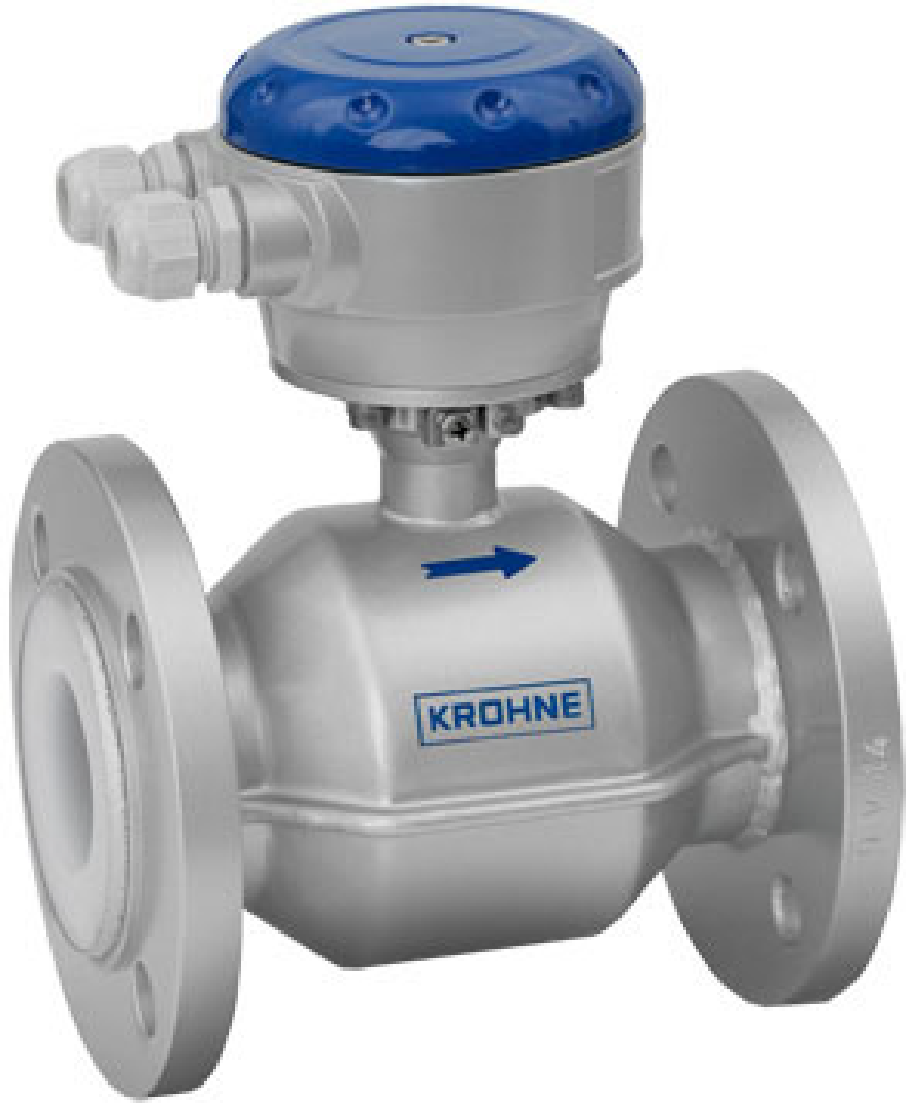
\includegraphics[width=1.8in,height=2.31944in]{figs/flowmeters/image1.png}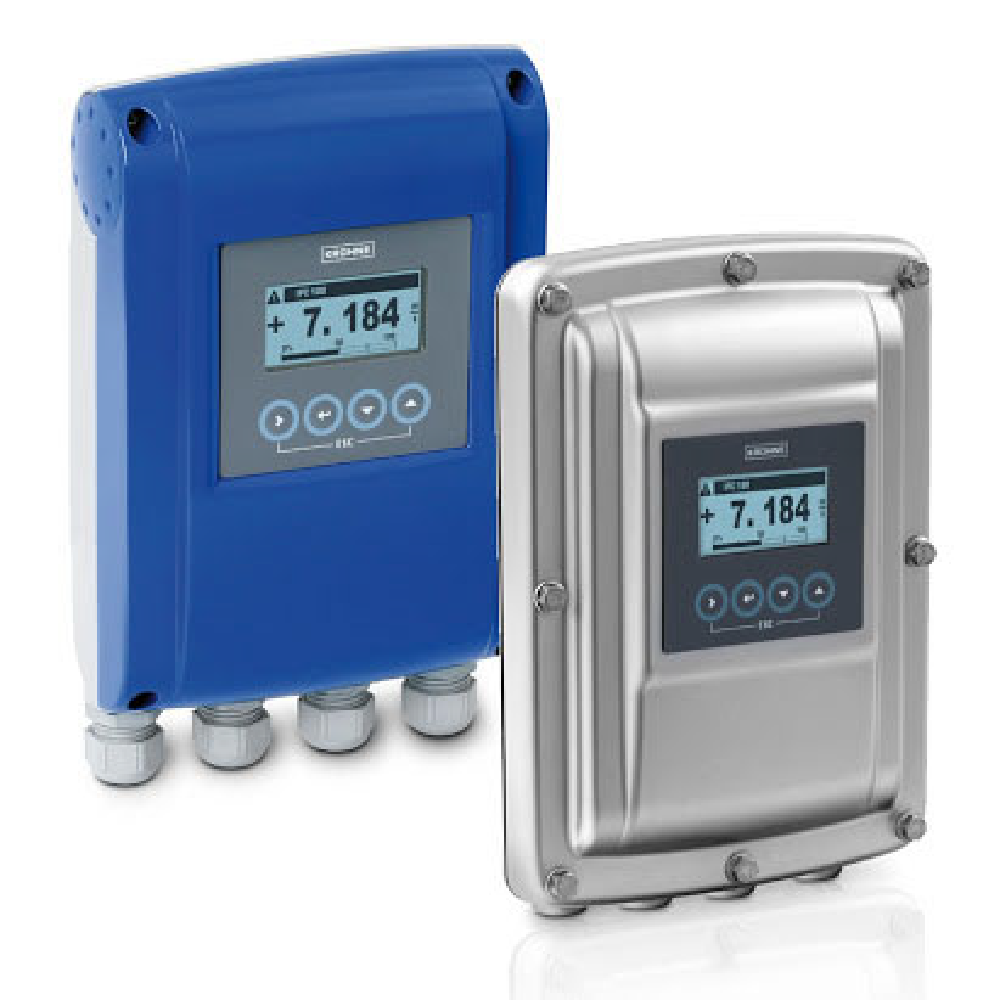
\includegraphics[width=2.0in,height=2.31944in]{figs/flowmeters/image2.png}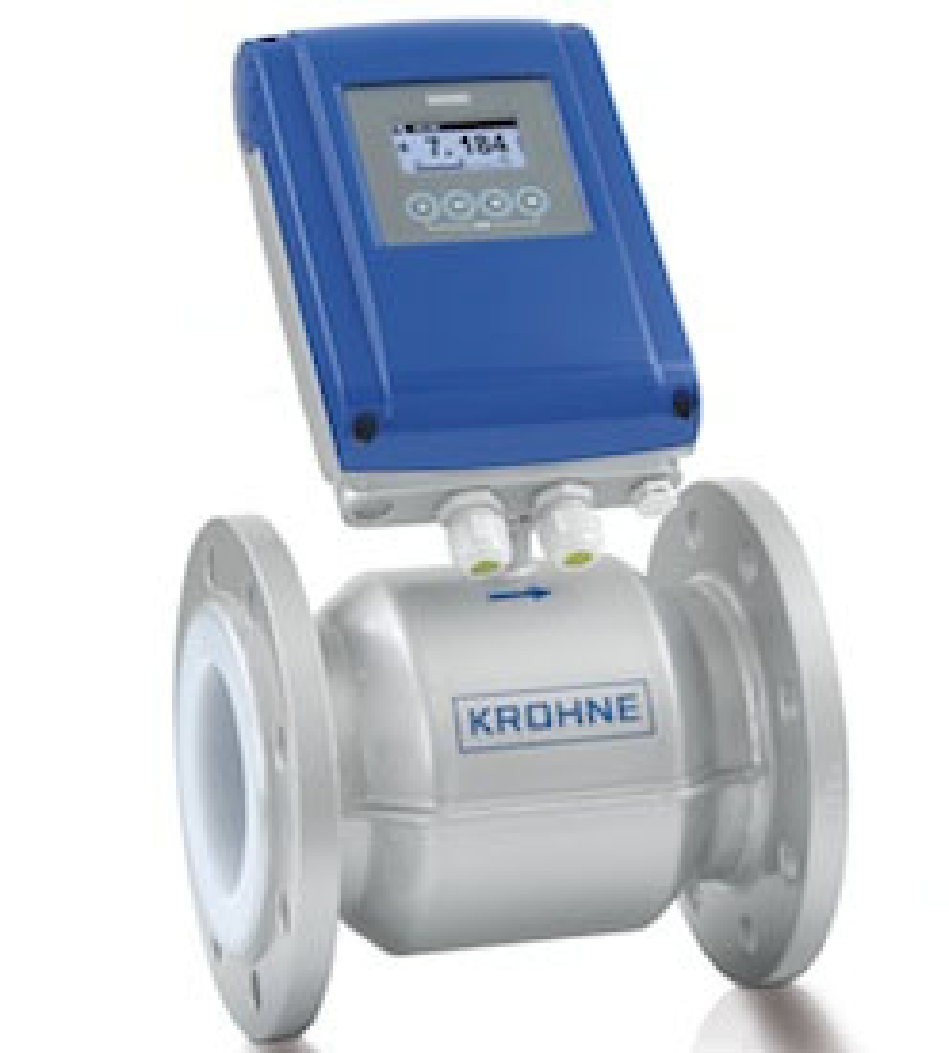
\includegraphics[width=2.0in,height=2.31944in]{figs/flowmeters/image3.png}
    \caption{Electromagnetic Flow Meters (a) Compact version; (b) Remote display.}
    \label{fig:ElectricFlowMETERS}
\end{figure}


Electromotive force (EMF) is induced in the fluid, which is directly
proportional to its velocity. By measuring this induced EMF, the flow
meter calculates the flow rate of the fluid. One of the primary
advantages of electromagnetic flow meters is their accuracy and
reliability, even in demanding industrial environments with fluctuating
flow rates, temperatures, and pressures. They have no moving parts,
which minimizes wear and tear, reduces maintenance requirements, and
ensures long-term stability and durability.

\subsection{Vortex Flow meter:}

A vortex flow meter is that type of flow meter which is used to assess
the flow rate of liquids, gasses, or steam in industrial applications.
It operates on the principle of the von Kármán effect, where vortices
are generated as a fluid flows past a bluff body installed into the flow
stream. These vortices alternate on either side of the bluff body, and
their frequency is directly proportional to the flow velocity.

The vortex flow meter detects these vortices using sensors, typically
piezoelectric sensors, and calculates the flow rate based on the
frequency of vortex shedding. Vortex flow meters provide advantages such
as its higher accuracy, wide turndown ratio, suitability for a variety
of fluids, and minimal pressure loss.

\begin{figure}[h!]
    \centering
    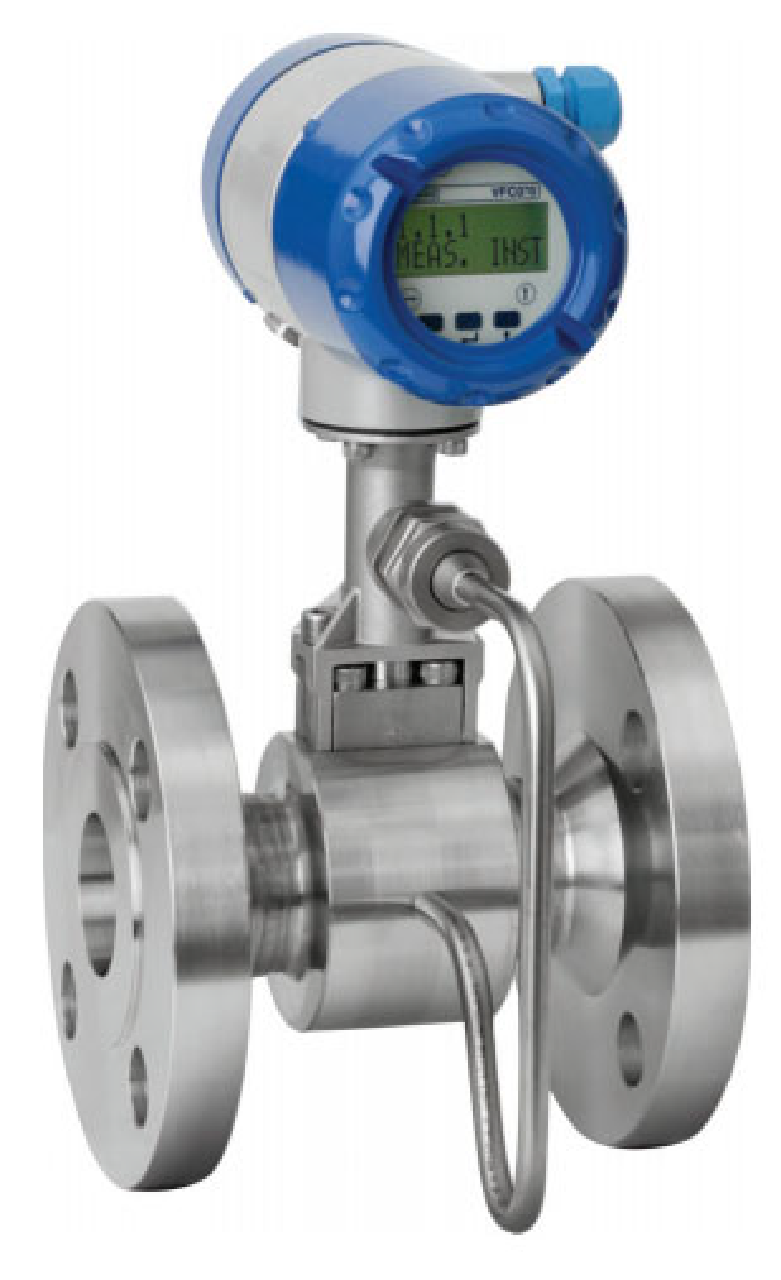
\includegraphics[width=1.41806in,height=2.31944in]{figs/flowmeters/image7.png}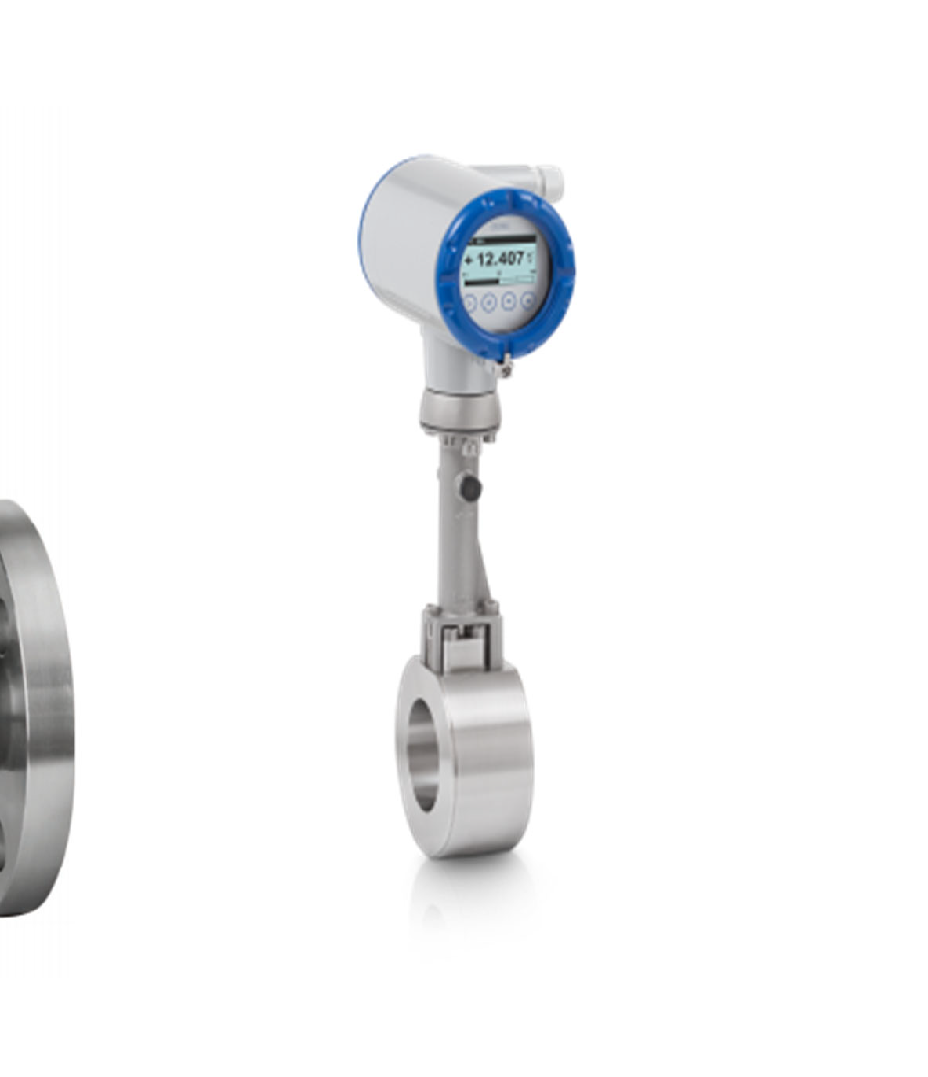
\includegraphics[width=1.99792in,height=2.31944in]{figs/flowmeters/image8.png}
    \caption{Various types of Vortex Flow Meters}
    \label{fig:electric_flowmeters}
\end{figure}

\subsection{Coriolis Mass Flow meter:}

A Coriolis mass flow meter is that type of flow meter which is used to
estimate the rate of flow of liquids or gases based on the Coriolis
effect. In this meter, the fluid flows through a vibrating tube or
tubes. As the fluid flows, it causes the tubes to twist due to the
Coriolis effect, which is a result of the fluid\textquotesingle s
inertia and the Earth\textquotesingle s rotation. Sensors detect this
twisting motion, and the amount of twist is directly proportional to the
mass flow rate of the fluid. Coriolis mass flow meters are known for
their high accuracy, wide turndown ratio, and ability to measure mass
flow directly, regardless of fluid properties such as density,
viscosity, or temperature.


\begin{figure}[h!]
    \centering
    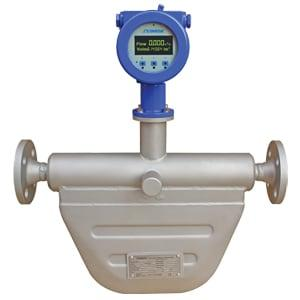
\includegraphics[width=2.31944in,height=2.31944in]{figs/flowmeters/image11.jpg}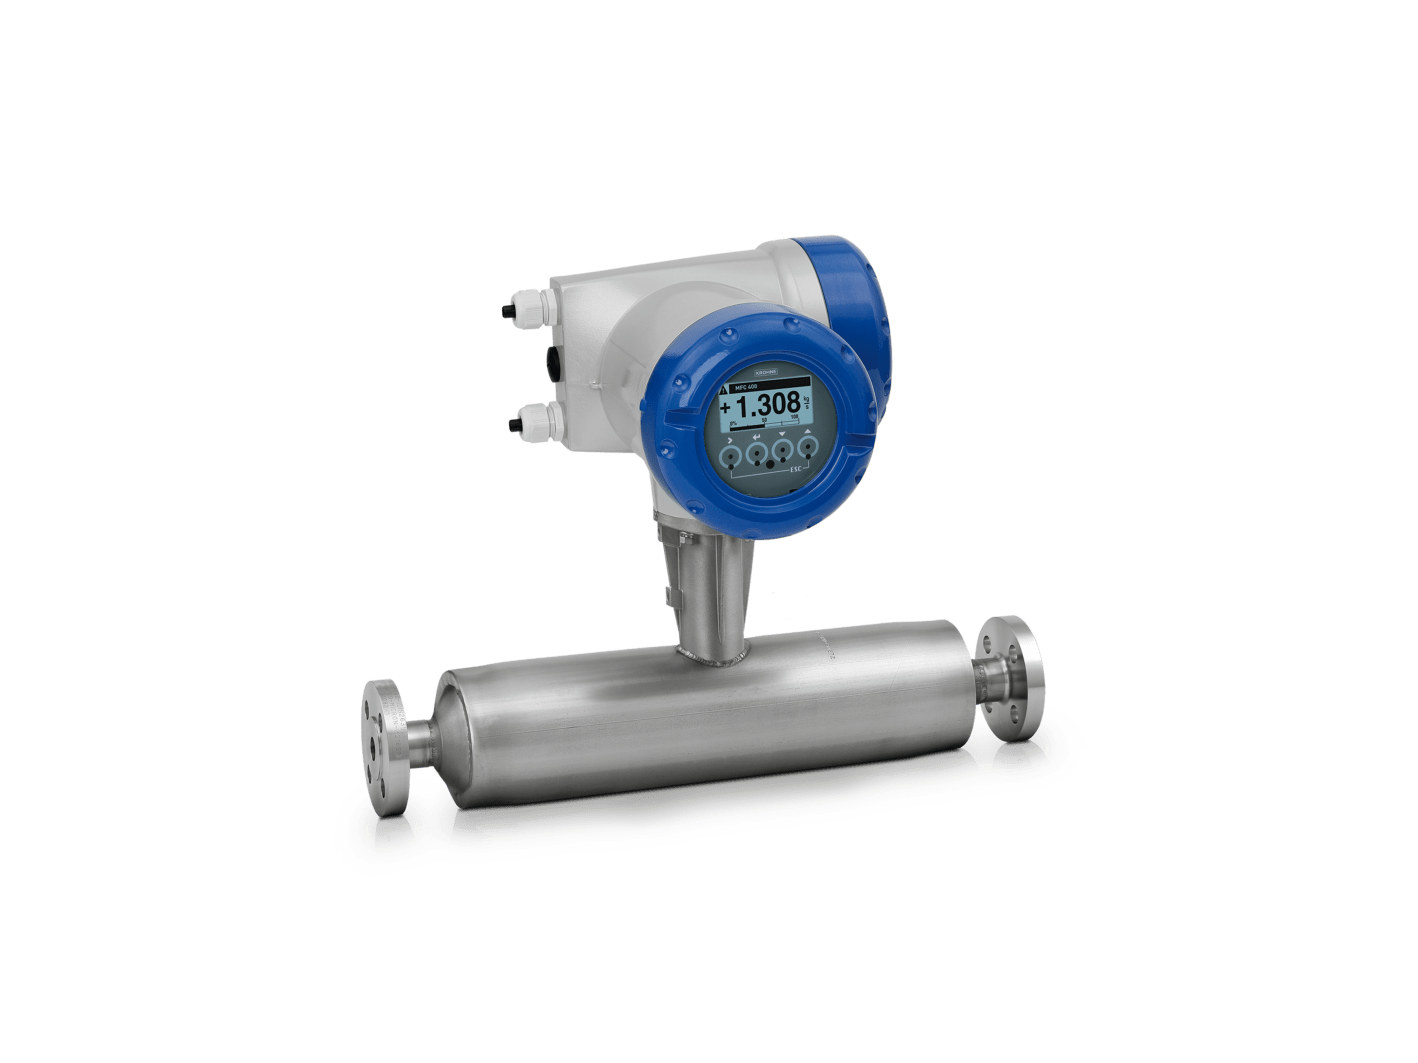
\includegraphics[width=3.09375in,height=2.31944in]{figs/flowmeters/image12.png}
    \caption{Various types of Coriolis Mass Flow meter.}
    \label{fig:Various types of Coriolis Mass Flow meter.}
\end{figure}

\subsection{Variable Area Flow meter:}

A variable area flow meter, also known as a Rota meter, is a type of
flow meter used to measure the flow rate of liquids or gases in
industrial applications. It consists of a tapered tube with a float
inside that moves vertically in response to the flow rate. As the flow
rate increases, the float moves upward, and as it decreases, the float
moves downward. The position of the float within the tapered tube
indicates the flow rate, with higher flow rates corresponding to higher
float positions.

\begin{figure}[h!]
    \centering
    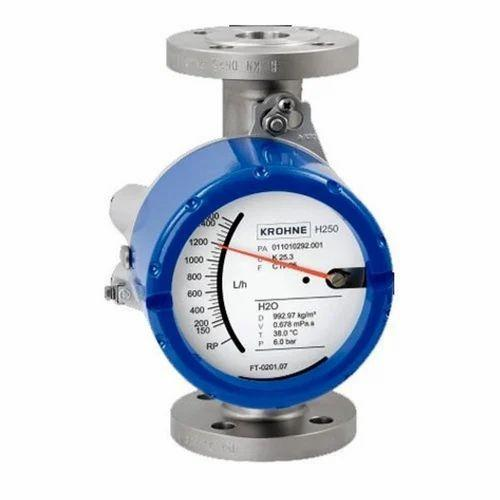
\includegraphics[width=0.45\linewidth]{figs/flowmeters/image15.jpg}
    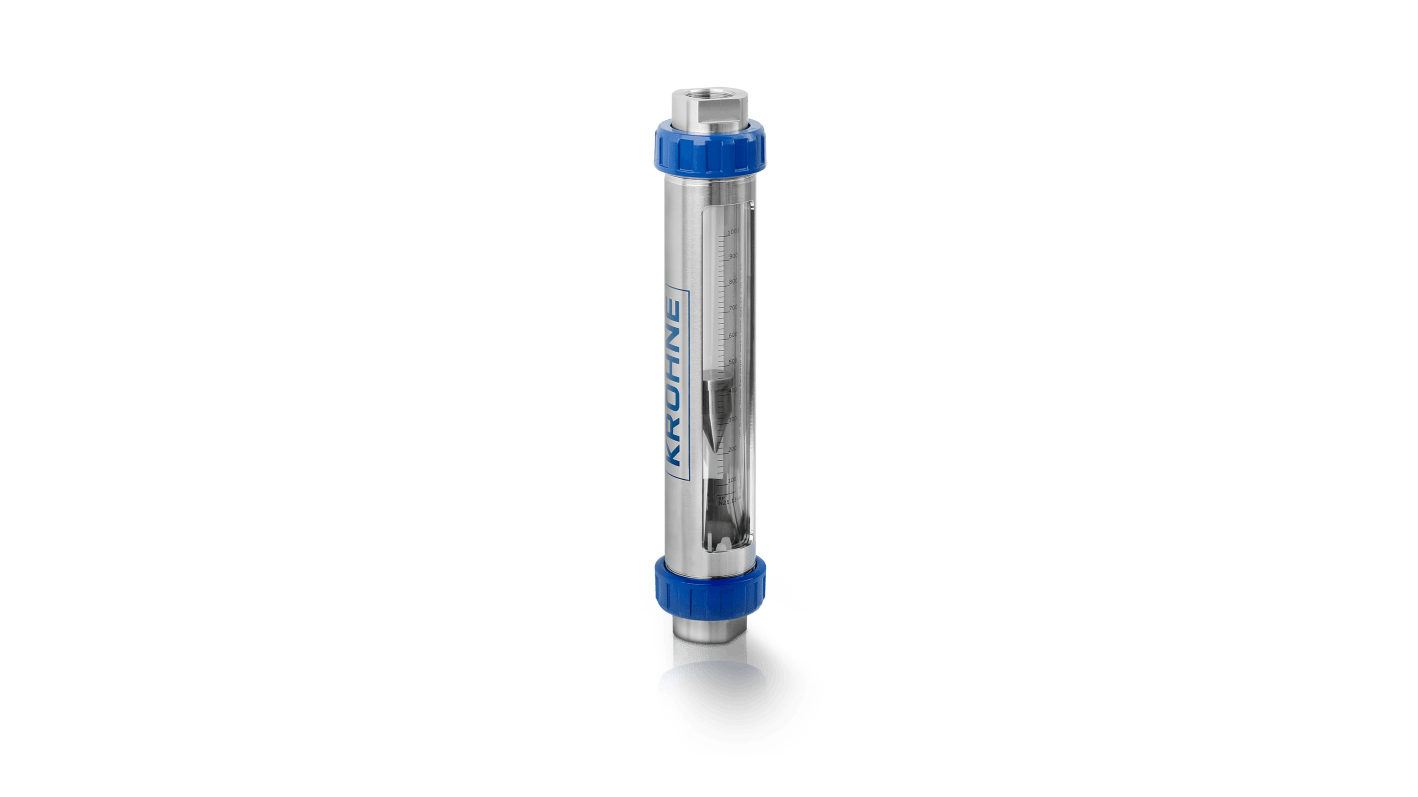
\includegraphics[width=0.8\linewidth]{figs/flowmeters/image16.png}
    \caption{Variable Area Flow Meters (Rota Meter)}
    \label{fig:rota_meter}
\end{figure}


Variable area flow meters are simple, cost-effective, and easy to
install. They offer visual indication of flow rate and can be used for
both high and low-pressure applications. However, their accuracy can be
affected by changes in fluid density, viscosity, and temperature.

\subsection{Orifice Type Flow meter:}

An orifice type flow meter is a commonly used differential pressure flow
meter which asses the rate of flow of liquids or gases in a pipeline. It
has a plate with a hole (or orifice) installed in the pipeline, creating
a pressure drop across the orifice plate as fluid flows through it.
Pressure taps located downstream and upstream of the orifice plate
measure the pressure differential, which is proportional to the flow
rate according to Bernoulli\textquotesingle s principle. By measuring
the pressure drop across the orifice plate, the flow rate can be
determined using empirical equations or calibrated charts. Orifice flow
meters are relatively simple, cost-effective, and suitable for a variety
of flow rates and fluid types. However, they can cause permanent
pressure loss in the system and may require frequent recalibration for
accurate measurements.


\begin{figure}[h!]
    \centering
    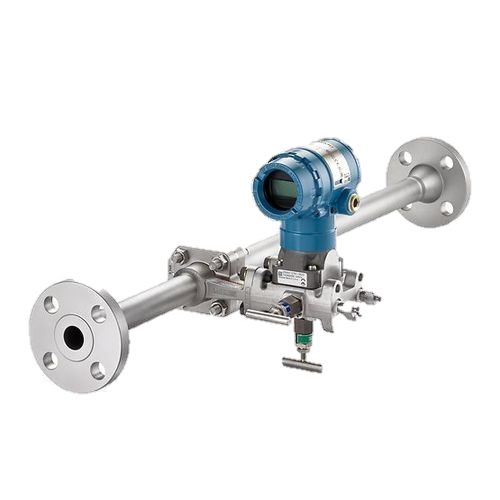
\includegraphics[width=0.8\linewidth]{figs/flowmeters/image19.png}
    \caption{Orifice type flow meter.}
    \label{fig:orifice_flow_meter}
\end{figure}


\subsection{Positive Displacement Flow meter:}

It is a type of flow meter that estimates the rate of flow of liquids by
repeatedly filling and emptying a chamber or chambers of known volume.
As the fluid flows through the meter, it displaces a known volume of
fluid, which is then estimated to calculate the flow rate.

\begin{figure}[h!]
    \centering
    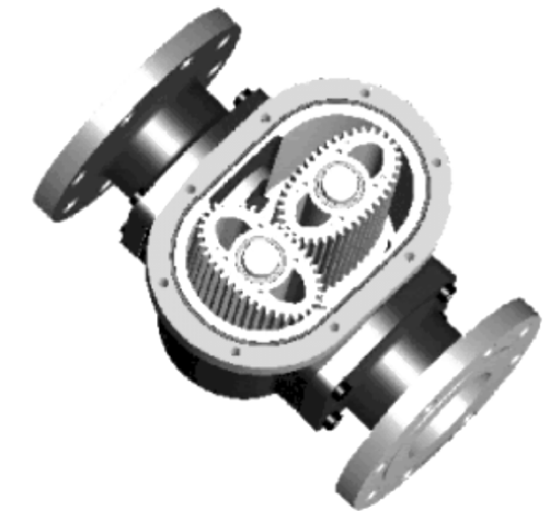
\includegraphics[width=2.50105in,height=2.32in]{figs/flowmeters/image20.png}
    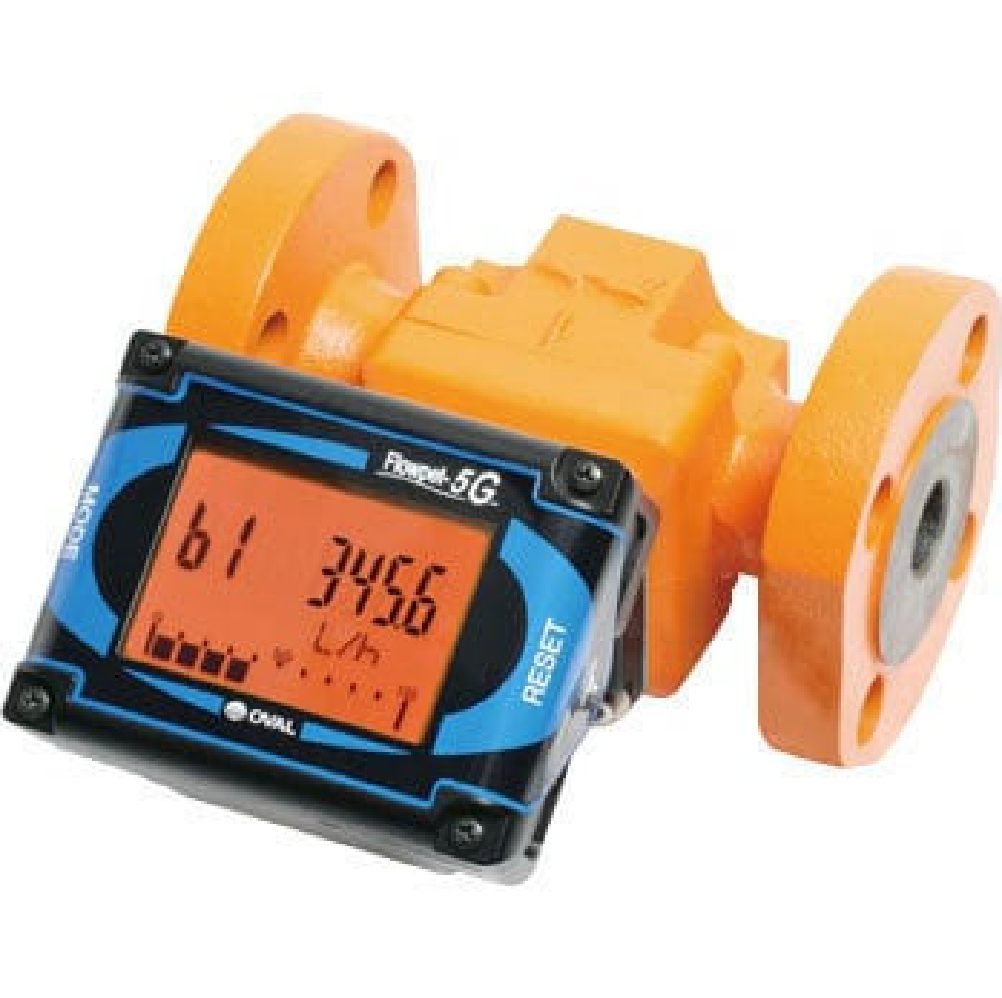
\includegraphics[width=2.33107in,height=2.32in]{figs/flowmeters/image21.png}
    \caption{Positive Displacement Flow meter}
    \label{fig:Positive Displacement Flow meter}
\end{figure}

\subsection{Open channel Flow meter:}

An open channel flow meter is a type of flow meter that estimates the
rate of flow of liquids in open channels, such as rivers, streams,
canals, or partially filled pipes. Unlike closed pipe flow meters, which
measure flow in pressurized pipes, open channel flow meters are designed
to measure flow in channels where the fluid surface is exposed to the
atmosphere. These meters typically use various methods to determine flow
rate, such as velocity-area method, ultrasonic sensors, or pressure
sensors.


\begin{figure}[h!]
    \centering
    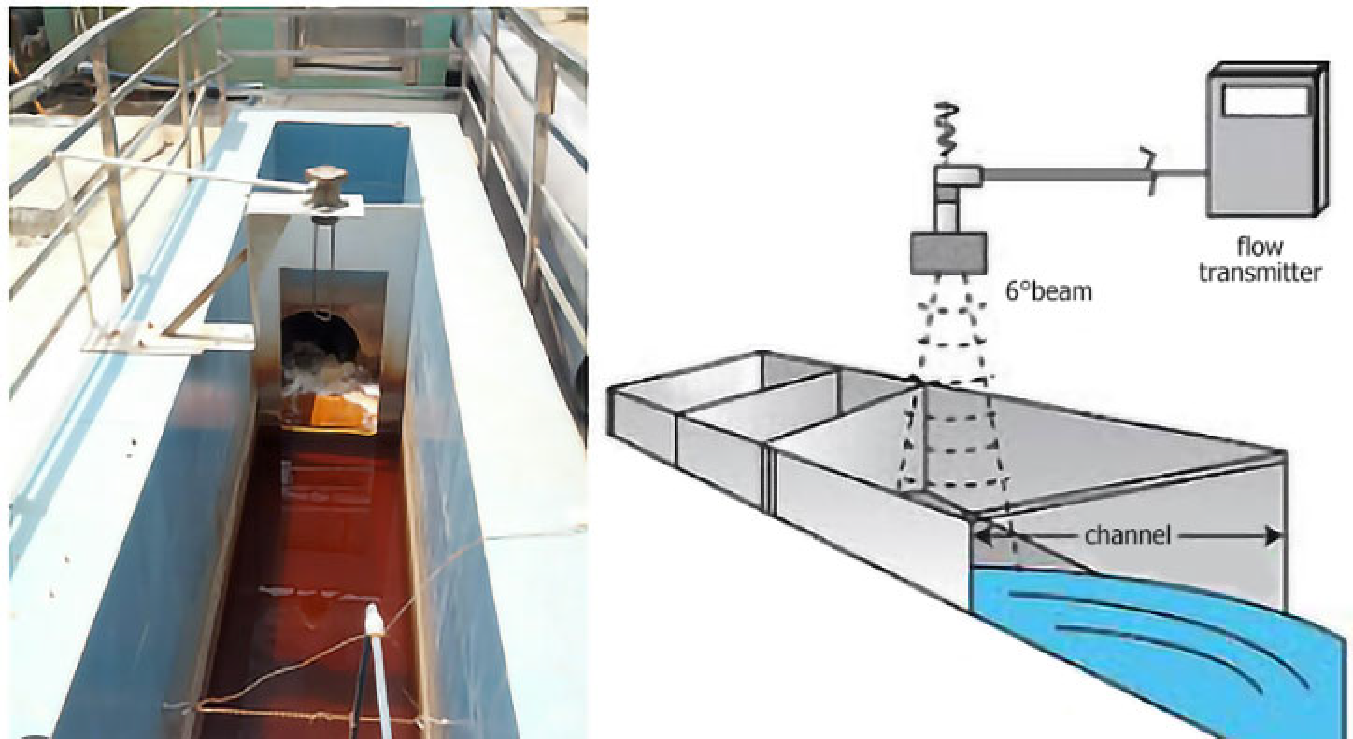
\includegraphics[width=0.8\linewidth]{figs/flowmeters/image22.png}
    \caption{Open channel flow meters}
    \label{fig:Open channel flow meters}
\end{figure}




\subsection{Turbine type Flow meter:}

It is a type of flow meter that estimates the rate of flow of liquids in
various industrial applications. It consists of a rotor with turbine
blades inserted into the flow stream. The fluid gives the turbine blades
kinetic energy as it passes through the meter, which causes them to
rotate. The rotation of the blades is proportional to the flow rate of
the fluid, allowing for accurate measurement of flow rate.

\begin{figure}[h!]
    \centering
    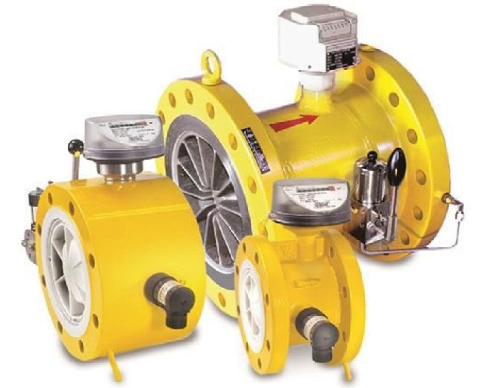
\includegraphics[width=2.18787in,height=1.76042in]{figs/flowmeters/image23.png}
    \caption{Turbine type flow meter.}
    \label{fig:Turbine type flow meter}
\end{figure}

